\documentclass{report}
\author{Samiran Das, 24B1270\\
Mentor \- Revanth Manepalli}
\usepackage{amsmath}
\usepackage{graphicx}
\title{SoS '25 Report\\
Control Systems}

\begin{document}

\maketitle

\chapter{Introduction}

\section{Definition:}
A Control System consists of subsytem and processes or plants assembled 
in such a way that we can obtain a desired performance given a specific input.

\begin{figure}[htbp]
    \centering
    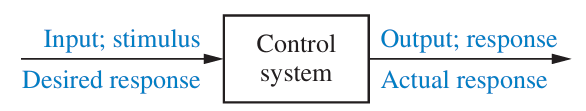
\includegraphics[scale=0.5]{images/cs_simple_bd.png}
    \caption{Simplified description of a Control System.}
\end{figure}

\section{Applications:}
Control systems make moving large equipments with insane precision possible.
An elevator reaching precisely leveled and alligned with the floor we input,
pointing huge antennas towards the farthest reaches of the universe precisely
to pick up faint radio signals are some examples of what we can achieve with well designed Control systems.
\par
We design control systems for four primary reasons:
\begin{itemize}
    \item \textbf{Power Amplification:} For example, the movement of a heavy piece of equipment is
    controlled by low-power input of a potentiometer or similar sensors and a large amount of power
    is required for output. A well designed control system can produce the required power amplification
    or power gain for it.
    \item \textbf{Remote Control:} 
\end{itemize}


\section{Open loop vs Closed loop systems}

\end{document}